\section{Method}
\label{sec:method}

Figure~\ref{fig:pipeline} summarizes the pipeline.

\begin{figure*}[t]
\centering
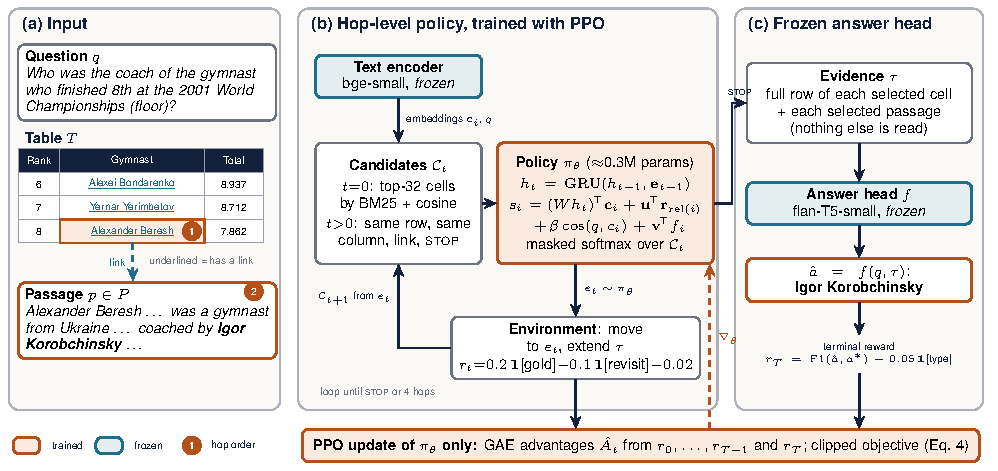
\includegraphics[width=\textwidth]{figures/architecture.pdf}
\caption{\hop\ architecture, shown on a HybridQA dev question. (a) Input: question, table and linked passages; numbers mark the hops taken. (b) The policy $\pi_\theta$, the only trained component, picks one candidate (cell, linked passage or \textsc{stop}) per hop; the environment returns the hop reward $r_t$ and the next candidate set. (c) On \textsc{stop}, the frozen answer head reads only the selected evidence $\tau$; its answer gives the terminal reward $r_T$. PPO updates $\pi_\theta$ from $r_0,\dots,r_T$. All path-based methods share every component except the learning signal.}
\label{fig:pipeline}
\end{figure*}

\subsection{Environment and candidates}
The encoder is the frozen sentence model \texttt{BAAI/bge-small-en-v1.5}; every entity and the question are embedded once and cached.
A cell is rendered as ``table title | column header | row anchor | cell text'', where the row anchor is the first non-numeric cell of the row; a passage is rendered as its title and first 400 characters.
At hop 0 the candidates are the top $K=32$ cells of the table by $0.5\cdot\mathrm{bm25}+0.5\cdot\cos(q,c)$ (BM25 min--max normalized within the table); STOP is illegal at $t=0$.
At later hops the candidates are all cells in the row of the current entity, the 8 cells of its column most similar to $q$, the passage linked from the current cell if there is one, and STOP.
A passage entity inherits the row and column of its source cell.
Re-selecting an entity is legal but flagged as redundant.
The episode ends on STOP, after $H=4$ selected entities (forced stop), or immediately on an illegal action.
The unrestricted variant A4 replaces the row/column neighbourhood at $t>0$ with the top-$K$ cells of the whole table by cosine similarity plus the linked passage and STOP.

\subsection{Policy}
The policy ($\approx$0.3M parameters, trained on CPU) keeps a GRU state $s_t$ over the embeddings of the selected entities, initialized as $s_0=\tanh(W_q q)$.
The logit of candidate $i$ with embedding $c_i$, relation type $\rho_i\in\{\text{start, same-row, same-column, link, stop}\}$ and feature vector $\phi_i$ is
\begin{equation}
\begin{split}\ell_i={}&(Ws_t)^\top c_i+u(s_t)^\top \mathrm{emb}(\rho_i)+\beta\cos(q,c_i)\\&+v^\top\phi_i+\tanh(F\phi_i)^\top g(s_t),\end{split}
\end{equation}
with illegal candidates masked before the softmax; a value head $V_\phi(s_t)$ is an MLP on $s_t$.
The features $\phi_i$ (Appendix~\ref{app:changes}) are the cosine similarity, the normalized BM25 score, the question-token overlap with the entity text and the question-token overlap with the column header (the last two lexical; passages have no BM25 score or header).
They are given identically to H1, A1--A4, B2a, B2b and, as a scorer input, to B3.

\subsection{Hybrid reward}
Let $g$ be the gold path.
For a legal hop that selects entity $e_t$:
\begin{equation}
\begin{split}r_t={}&w_{\text{hop}}\,\mathbb{1}[e_t\in g,\ \text{ordered, new}]\\&-w_{\text{red}}\,\mathbb{1}[e_t\text{ revisited}]-w_{\text{step}}.\end{split}
\end{equation}
\emph{Order-consistent} means the gold index of $e_t$ is not smaller than the largest gold index matched so far; a revisit never re-earns $w_{\text{hop}}$ (an exploit found and fixed during review).
STOP itself earns nothing.
At termination, with $\hat a=f(q,\tau)$,
\begin{equation}
\begin{split}r_T={}&w_{\text{ans}}\,\mathrm{F1}(\hat a,a^\ast)\\&-w_{\text{schema}}\,\mathbb{1}[\text{last cell schema-inconsistent}].\end{split}
\end{equation}
The schema rule uses fixed question cues: a cue such as ``how many'' or ``percent'' requires the last selected cell to have numeric type, and a date cue such as ``what year'' requires a date or number; questions without a cue impose no constraint, and passages are never penalized.
For questions without a gold path ($1.7\%$ of all questions, Appendix~\ref{app:data}) the hop term is zero.
Default weights are $w_{\text{ans}}=1$, $w_{\text{hop}}=0.2$, $w_{\text{red}}=0.1$, $w_{\text{schema}}=0.05$, $w_{\text{step}}=0.02$ and were fixed before training (Table~\ref{tab:reward-weights}).

\subsection{PPO training}
We use a custom clipped-objective PPO with GAE ($\gamma=1$, $\lambda=0.95$), clip $0.2$, value coefficient $0.5$, entropy coefficient $0.01$ decayed linearly to zero, 4 epochs of minibatches of 256 steps per update, per-batch advantage normalization, gradient-norm clipping at $0.5$, Adam with learning rate $3\times10^{-4}$, and 64 single-trajectory episodes per update.
The terminal reward is added to the last step of each trajectory.
The training budget is 48{,}000 trajectories (750 updates).
Variants A1--A4 change only the reward switches or the action space: A1 uses the terminal answer reward only, A2 removes the redundancy penalty, A3 removes the schema term and A4 uses the unrestricted action space.

\subsection{Frozen answer head and row evidence}
The answer head is \texttt{google/flan-t5-small}, fine-tuned once on gold-path evidence (3 epochs, learning rate $3\times10^{-4}$) with distractor entities inserted into 30\% of training examples so that it tolerates imperfect selections, and then frozen for all path-based methods.
Its input is ``question: $q$ evidence: $x_1\,\|\,x_2\dots$'' truncated to 512 tokens, where the evidence $x_j$ is the rendering of the selected entities.
In the final configuration (Appendix~\ref{app:changes}) every selected cell is rendered as its whole row, once per row in first-visit order, and every selected passage as its title and text; passages enter the input only if the policy selects them.
Hence the answer head can read the answer from the row of a selected cell, and a policy that selects a good first cell can already earn answer reward, whereas passage answers require the link hop.
